
\documentclass[letterpaper, 10pt, conference]{ieeeconf} 


\IEEEoverridecommandlockouts 

\overrideIEEEmargins

\usepackage{enumerate}
\usepackage{graphicx}
\usepackage{amsmath, amssymb}%,amsthm}

\usepackage{framed}
\usepackage{url}
%\usepackage{hyperref}

\newtheorem{thm}{Theorem}
\newtheorem{example}{Example}
\newtheorem{prop}{Proposition}
\newtheorem{lemma}{Lemma}
\newtheorem{corollary}{Corollary}

%\theoremstyle{definition}
\newtheorem{alg}{Algorithm}
\newtheorem{assumption}{Assumption}
\newtheorem{definition}{Definition}
\newtheorem{problem}{Problem}

\usepackage{ifthen,version}
\newboolean{include-notes}
% Comment out the following line to exclude the notes.
\setboolean{include-notes}{true}
%notes
\newcommand{\tcnote}[1]{\ifthenelse{\boolean{include-notes}}%
 {\textbf{TC says: #1}}{}}

\newboolean{show-removed}
\setboolean{show-removed}{false}
\usepackage{color}
\newcommand{\removed}[1]{\ifthenelse{\boolean{show-removed}}%
  {{\color{red} #1}}{}}


\newboolean{show-proofs}
\setboolean{show-proofs}{true}
\newcommand{\showproof}[1]{\ifthenelse{\boolean{show-proofs}}%
  {#1}{}}



\DeclareMathAlphabet{\mathpzc}{OT1}{pzc}{m}{it}
\DeclareFontFamily{U}{msb}{}
\DeclareFontShape{U}{msb}{m}{n}{ <5> <6> <7> <8> <9> gen * msbm
<10> <10.95> <12> <14.4> <17.28> <20.74> <24.88> msbm10}{}
\DeclareSymbolFont{AMSb}{U}{msb}{m}{n}
\DeclareMathSymbol{\Reals}{\mathalpha}{AMSb}{'122}
\DeclareMathSymbol{\Naturals}{\mathalpha}{AMSb}{'116}
\DeclareMathSymbol{\Knumbers}{\mathalpha}{AMSb}{'113}
\DeclareMathSymbol{\Rationals}{\mathalpha}{AMSb}{'121}
\DeclareSymbolFont{AMSb}{U}{msb}{m}{n}
\DeclareMathSymbol{\setB}{\mathalpha}{AMSb}{'102}
\DeclareMathSymbol{\setC}{\mathalpha}{AMSb}{'103}
\DeclareMathSymbol{\setD}{\mathalpha}{AMSb}{'104}
\DeclareMathSymbol{\setE}{\mathalpha}{AMSb}{'105}
\DeclareMathSymbol{\setF}{\mathalpha}{AMSb}{'106}
\DeclareMathSymbol{\setI}{\mathalpha}{AMSb}{'111}
\DeclareMathSymbol{\setK}{\mathalpha}{AMSb}{'113}
\DeclareMathSymbol{\setM}{\mathalpha}{AMSb}{'115}
\DeclareMathSymbol{\setN}{\mathalpha}{AMSb}{'116}
\DeclareMathSymbol{\setP}{\mathalpha}{AMSb}{'120}
\DeclareMathSymbol{\setQ}{\mathalpha}{AMSb}{'121}
\DeclareMathSymbol{\setR}{\mathalpha}{AMSb}{'122}
\DeclareMathSymbol{\setS}{\mathalpha}{AMSb}{'123}
\DeclareMathSymbol{\setT}{\mathalpha}{AMSb}{'124}
\DeclareMathSymbol{\setU}{\mathalpha}{AMSb}{'125}
\DeclareMathSymbol{\setV}{\mathalpha}{AMSb}{'126}
\DeclareMathSymbol{\setW}{\mathalpha}{AMSb}{'127}
%\DeclareMathSymbol{\setX}{\mathalpha}{AMSb}{'128}
%\DeclareMathSymbol{\setY}{\mathalpha}{AMSb}{'129}
\DeclareMathSymbol{\setX}{\mathalpha}{AMSb}{'130}
\DeclareMathSymbol{\setY}{\mathalpha}{AMSb}{'131}
\DeclareMathSymbol{\setZ}{\mathalpha}{AMSb}{'132}

\title{Optimal Parameter Identification for Discrete Mechanical Systems with Application to Flexible Object Manipulation}


\author{T. M. Caldwell and  D. Coleman and N. Correll% <-this % stops a space
\thanks{
This material is .....}%
}

\begin{document}
\maketitle

\begin{abstract}
%This paper considers the problem of optimal parameter identification of flexible objects using variational integrators for simulation.  The example object is 



%We provide a discrete-time adjoint-based gradient calculation 

 %and apply it to identifying the stiffness properties of a flexible loop.  
\end{abstract}

\section{Introduction}
The goal of this works is to use a robotic arm to identify the behavior of a flexible object through touch only.  The object under consideration for this paper is a flexible loop.  We assume the robot has already rigidly grasped the object at one end and that it is clamped at the other.  The robot then bends, twists and stretches the loop.  During the manipulation, the robot measures the arm's joint torques and joint angles.  With this information, it is possible to back out mechanical properties of the loop in order to generate an accurate model for future control and manipulation.  In this paper, the manner in which we model the loop is so that the underlying mechanics of the loop are the same as the robot arm.  Furthermore, we provide an optimal control approach for calculating properties of the model that best matches the behavior of the physical loop.

There are many methods to model and simulate flexible objects \cite{khalil_payeur}.  A common approach is to model the object as a lattice or collection of links of masses and springs \cite{sahari_etal, wakamatsu_etal}\textbf{cite others?}.  This approach has been done for simulation of linear object like strings, hair, and electrical cables which have a series of masses linked together with springs.   Our approach is similar with the primary difference that the loop connects back onto itself.  This connection restricts the loops movement and is handled using holonomic constraints.  

We approximate the loop as a ring of $n_l$ links.  Adjacent links connect together through spherical joints with torsional springs. We assume each link is rigid and as such the vast theory of rigid body mechanics is relevant \cite{murray_li_sastry}.  Furthermore, since the robot arm is a series of joined rigid links---albeit with actuated joints---the full system, robot arm and loop, can be modeled together.  As such, planning and control can be done in the configuration space, instead of the end effector or object space. 

\begin{figure}
\centering
\includegraphics[width = 250pt]{bloop_image_1.pdf}
\caption{Illustration of Rethink Robotics' Baxter manipulating the approximated loop.}
\label{fig-baxter_image_1}
\end{figure}

We use Rethink Robotics' Baxter robot to both manipulate and measure the loop.  Each of Baxter's arms have 7 degrees of freedom.  The arms are designed for compliance since each joint has a series elastic actuators that allows for force sensing and control.  An illustration of Baxter manipulating a six link approximation of a loop is in Figure~\ref{fig-baxter_image_1}

A good representation of the flexible object is not enough to accurately model a flexible object.  We also need the model simulation to be consistent with the physical behavior of the loop.  We decided not to apply Euler integration or another low order integrator to the continuous dynamics, as is the case in \cite{sahari_etal}, because such integrators can introduce significant energy errors.  At worst these errors will destabilize the integration and at best compromise the model's energy dissipation \cite{johnson_murphey_scalable}.  Instead we decided to use \emph{variational integrators}.  Variational integrators are designed from the least action principle and have good properties that match known physical phenomenon like preserving---or nearly preserving---conservation of energy and momentum \cite{johnson_murphey_scalable, marsden_west}.

Furthermore, variational integrators elegantly handle holonomic constraints.  Holonomic constraints are specified as $h(q) = 0$, where $q$ is the system's configuration.  They are used to constrain positions and orientations.  For the example, we use holonomic constraints to ``close the loop''---i.e. to constrain the link at one end of the loop to the other end.  In simulating continuous dynamics holonomic constraints are handled with equivalent constraints on the acceleration that creep due to numerical integration error.  In comparison, variational integrators apply holonomic constraints directly and do not have this issue (see \cite{johnson_murphey_scalable} for a discussion).

Due to recent work by Johnson and Murphey \cite{johnson_murphey_scalable, johnson_murphey_linearization}, it is possible to efficiently simulate mechanical systems using variational integrators in generalized coordinates. They provide a framework using a tree representation and caching that not only makes for efficient simulation---especially for articulated rigid bodies---but also efficient model based calculations like linearizations about a trajectory.   In optimal controls, linearizations are needed for gradient calculations like the gradient calculation presented in this paper.  %As such, we review mechanical systems, variation integrators and give the system Jacobian as derivatives of the system's Lagrangian and forcing. 

With a model and simulation that accurately predicts the motion of a flexible object, unknown quantities of its behavior, referred to as system parameters, can be identified.  These system parameters may be lengths, masses, or damping coefficients.  For the example, we assume the loop's stiffness is unknown.  As such, the goal is to obtain the spring constants of the torsional springs at the loop model's joints.  In this paper, this is done using an optimal control type approach.





%This paper considers the problem of optimal parameter identification for mechanical systems described by variational integrators.  The motivating example is a flexible loop clamped at one end and manipulated at the other.  By stretching, twisting, and bending the loop, the manipulator displaces the point of contact.  With the displacement measurement, along with the torques and forces that affected the displacement, the stiffness properties of the loop can be identified.  The identification approach is an optimal one for which we provide an adjoint-based gradient calculation.

%We model the loop as six links forming a hexagon.  The links connect together through spherical joints attached with torsional springs.  The goal of the example is to identify the torsional springs' spring constants.   Alternatively, other parameters could be identified like lengths, masses, and damping coefficients.  The presented approach also extends to identification of the coefficient of friction of a system's interaction with a surface similar to \textbf{cite Miller}.  %  A holonomic constraint is needed to constrain the loop's beginning and end frames to the same position and orientation in order to ``close the loop''.  

%Although we are concerned with flexible objects, we model them as connected rigid bodies for which modeling techniques are well understood \textbf{cite murray li sastry}.  For this reason, the presented parameter identification approach makes use of standard rigid body modeling techniques \textbf{cite Murray Li Sastry}.  Furthermore, we use variational integrators for simulation in order to provide a means to preserve\textemdash or nearly preserve\textemdash physical properties like conservation of energy and momentum \textbf{cite West Thesis, Johnson scalability, others...} \textbf{Johnson cites J. E. Marsden and M. West, “Discrete mechanics and variational integrators,” Acta Numer., vol. 10, pp. 357–514, 2001}.  This decision was made because simulation accuracy is a concern for lower order integrators which can significantly introduce energy errors.  At worst these errors will destabilize the integration and at best compromise the model's dissipation \textbf{cite Johnson's scalability paper}.  

%Numerical issues are exacerbated for systems with closed chains---which is the case for the motivating example---since numerical error during Simulation can invalidate holonomic constraints. This problem arises due to the way holonomic constraints are included in continuous dynamics, which is with equivalent acceleration constraints.  In comparison, variational integrators apply the holonomic constraints directly and do not have this issue \textbf{Johnson and Murphey scalable}.



The parameter identification optimization problem is set up as a discrete-time Bolza type problem.  For the loop example, the cost function is a summation of the joint errors between the simulated joint angles for a given set of parameters and the measured joint angles.  The joint error directly correlates to the difference between the simulated loop displacement and the measured loop displacement, at least at the manipulator   Alternatively, the cost can be given by a maximum likelihood estimate for which the cost is lower for parameters that correspond to the simulation that is most consistent with the measurement (see \cite{houska_etal}).  

The paper's contributions are twofold.  First, it provides a discrete-time adjoint-based gradient calculation for optimal parameter estimation.  Second, it formulates physical parameter identification of flexible objects with variational integrators for greater confidence in the accuracy of the model's simulation.

This paper is organized as follows: ..........

% They implement the variational integrator and efficient linearization in an open source software package for articulated rigid body mechanical systems\textemdash see TREP \textbf{cite}. 



%A system parameter is a feature of the system that is fixed during the evolution of the system.  For example, we may wish to estimate the lengths, masses, stiffnesses, and damping coefficients of physical links of a system.  Or, we may wish to estimate the coefficient of friction of a system's interaction with a surface as in \textbf{cite Miller}.  

%The proposed parameter estimation calculates the system parameters with corresponding simulation that best matches measured data.  The optimization problem is set up as a Bolza problem.  In the examples, we choose a cost that is quadratic in the error of the simulated state with the measured state for a given parameter.  Alternatively, the cost can be given by a maximum liklihood estimate for which the cost is lower for parameters with greater probability of being true given the measurement (see \textbf{cite parameter estimation book and houska}).  

%We provide an adjoint-based calculation for the gradient of the cost with respect to the parameters which can be used in an iterative optimization procedure like steepest descent.  The gradient depends on the linearization of the equations of motion.  As such, we review mechanical systems and give the system Jacobian as derivatives of the system's Lagrangian and forcing.  



%\subsection{Why is this hard?}
%Model based parameter estimation for complex mechanical systems have a number of complications.  First, simulation accuracy and computation speed are inversely related.  A lower order integrator can significantly introduce energy errors which at the worst will destabilize the integration and at best compromise dissipation parameter estimation \textbf{cite Johnson's scalability paper}.  The problem is exacerbated for systems with closed chains since numerical error can invalidate holonomic constraints.  A higher order integrator is not a desirable alternative because the higher the order, the more intermediate computations needed to calculate each integration step which makes for slower execution.

%Second, automated model based calculations like linearization evaluations about a trajectory can scale poorly with the number of states and controls---especially for articulated systems.  The straightforward method to calculate the Jacobian symbolically is impractical for sufficiently complex mechanical systems, which is largely due to applications of chain rule.  Indeed, even for many complex systems, simply storing the symbolic representation of the equations is impractical or even infeasible.

%Fortunately, variational integrators \textbf{cite West Thesis, Johnson scalability, others...} provide a means to preserve\textemdash or nearly preserve\textemdash physical properites like conservation of energy and momentum \textbf{Johnson cites J. E. Marsden and M. West, “Discrete mechanics and variational integrators,” Acta Numer., vol. 10, pp. 357–514, 2001}.  Furthermore, Johnson and Murphey provide a framework using a tree representation and caching that not only makes for efficient simulation \textbf{cite Johnson scalability} but also efficient linearization evaluation \textbf{Johnson linearization}.  They implement the variational integrator and efficient linearization in an open source software package for articulated rigid body mechanical systems\textemdash see TREP \textbf{cite}. 

%Variational integrators give reason to expect the mechanical system simulation does not violate physical properties while the scalable formulation give reason to expect the necessary calculations like linearization evaluations can be done in a reasonable time. It is worth noting that variational integrators are not limited to just conservative systems.  They can handle forcing and dissipation.  They also handle holonomic constraints directly which avoids numerical error in the simulation violating the constraint \textbf{cite}. Ideally, simulation is sufficiently accurate as to not be the cause for error in the parameter estimation and it is sufficiently fast as to not be a reason for not doing the estimation in the first place.





\section{Mechanical Systems}
\label{sec-sim}
A comparison of continuous time and discrete time mechanical systems is presented.  The mechanical system depends on $n_a$ system parameters from the parameter space $\mathcal{A}\in\setR^m$. The mechanical system has $n_q$ generalized coordinates $q\in\setR^{n_q}$.  For continuous time, $q$ varies the continuous variable $t$\textemdash e.g. $q(t)$\textemdash for $t$ in the interval $[0,t_f]$, $t_f>0$.  Likewise, for the discrete representation, $q$ varies with the discrete variable $k$\textemdash e.g. $q_k$\textemdash for $k$ in the set $\mathcal{K}:=\{0,1,\ldots,k_f\}$, $k_f>0$.  Each discrete time $k$ pairs with a continuous time, labeled $t_k$, where $t_0 = 0$, $t_{k_f} = t_f$ and $t_k<t_{k+1}$. This section presents the continuous and discrete dynamics dependent on the parameters $a\in\mathcal{A}$.  The continuous dynamics are provided for comparison with the discrete system, in which the paper results are given.

\subsection{Continuous Mechanical System}
We review continuous mechanical systems for reference with discrete mechanical systems.  

A mechanical system's evolution is given by the path of least action.  The system's action is 
\[
S = \int_0^{t_f}L(q(\tau),\dot{q}(\tau),a)d\tau
\]
where $L(q,\dot{q},a) := KE(q,\dot{q},a) - V(q,a)$, the system Lagrangian, is the difference of the system's kinetic energy, $KE$, with its potential energy, $V$.  For this paper, we assume that both kinetic and potential energies depend on system parameters $a\in\mathcal{A}$.  Possible parameters of $L$ are lengths, spring constants, and masses. 

As is common in mechanical systems, we wish to include external forces, $F_c(q,\dot{q},a,t)$.  This term is the total external forcing in the generalized coordinates.  We also assume dependence on parameters $a\in\mathcal{A}$.  For example, likely parameter candidates showing in $F_c$ are damping coefficients.  By including the additional external force term, $F_c$, to the action, the Lagrange d'Alembert principle finds that the continuous dynamics of the mechanical system are given by the forced Euler-Lagrange equations \textbf{cite}:
\[
\frac{d}{d t}\frac{\partial}{\partial \dot{q}}L(q,\dot{q},a) - \frac{\partial}{\partial q}L(q,\dot{q},a) = F_c(q,\dot{q},a,t).
\]
Holonomic constraints can be enforced as external forces using Lagrange multipliers.  The $n_h$ holonomic constraint equations are given in the form $h(q,a)= [h_1,\ldots,h_{n_h}]^T(q,a) = 0$.  With the addition of the constraint, the forced Euler-Lagrange equations are \textbf{cite}:
\begin{equation}
\begin{array}{c}
\frac{d}{d t}\frac{\partial}{\partial \dot{q}}L(q,\dot{q},a) - \frac{\partial}{\partial q}L(q,\dot{q},a) = F_c(q,\dot{q},a,t) + \frac{\partial}{\partial q}h^T(q,a)\lambda\\
\frac{\partial^2}{\partial q^2}h(q,a)\circ(\dot{q},\dot{q}) + \frac{\partial}{\partial q}h(q,a)\ddot{q} = 0 
\end{array}
\label{eq-cont_EL}
\end{equation}
where $\lambda(t)\in\setR^{n_h}$ are Lagrange multipliers.  For fixed parameters $a$, the system's evolution is integrated from Eq.(\ref{eq-cont_EL}) for $q$, $\dot{q}$ and $\lambda$.  It is worth noting that holonomic constraints are not enforced directly but instead the acceleration is constrained.  During integration, numerical error will violate the constraint and $h(q,a)\neq 0$.

Equation \ref{eq-cont_EL} can be transformed into first-order state space equations.  Define the continuous state as $x = [q,\dot{q}]^T$.  The state equations, dependent on the parameters $a\in\mathcal{A}$, are $\dot{x}(t) = f(x(t),\lambda(t),a,t)$ where $\ddot{q}$ is specified by the forced Euler-Lagrange equations.  In the state space representation, gradient and Hessian calculations with respect to parameters are given for parameter optimization in \textbf{cite Lauren}.
%The term $F_c$ is the total external forcing in the generalized coordinates, which we also assume depends on parameters $a\in\mathcal{A}$.  The parameters $a$ could be, for instance, the coefficients of friction for a sliding system or the spring factors characterizing a system's stiffness.

\subsection{Discrete Mechanical System}
The discrete mechanical system is an approximation of its continuous counterpart.  For an initial configuration $q(0)$ and velocity $\dot{q}(0)$, the continuous configuration $q([0,t_f])$ is integrated from the forced Euler-Lagrange equations, Eq.(\ref{eq-cont_EL}).  The discrete analog to the forced Euler-Lagrange equations instead calculates the sequence $q_k\approx q(t_k)$ using a variational integrator approach \textbf{cite}.  

The discrete Lagrangian, labelled $L_d$, is an approximation of the action over a short time interval.  Instead of a velocity term, the discrete Lagrangian is defined by the current and next configurations, $q_k$ and $q_{k+1}$:
\begin{equation}
L_d(q_k,q_{k+1},a) \approx \int_{t_k}^{t_{k+1}}L(q(\tau),\dot{q}(\tau),a)d\tau.
\label{eq-Ld}
\end{equation}
The integration can be approximated with a quadrature like midpoint or trapezoidal rules.  Refer to \cite{johnson_murphey_scalable} for details of using midpoint rule, which we use in the example.  

Similarly, external forcing is included by approximating $F_c$ by the discrete left and right forces $F_d^-(q_k,q_{k+1},a,t_k,t_{k+1})$ and $F_d^+(q_k,q_{k+1},a,t_k,t_{k+1})$ using a quadrature.  In addition, the $n_h$ holonomic constraints $h(q_k,a)$ can be enforced with the $n_h$ Lagrange multipliers $\lambda_k$.  With the discrete Lagrangian, discrete forces and holonomic constraints, \cite{johnson_murphey_scalable}, finds that the forced discrete Euler-Lagrange equations are:
\begin{equation}
\left\{\begin{array}{l}
D_2 L_d(q_{k-1},q_{k},a) + F_d^+(q_{k-1},q_{k},a,t_{k-1},t_{k}) \\\hspace{20pt}+ D_1L_d(q_k,q_{k+1},a) + F_d^-(q_k,q_{k+1},a,t_k,t_{k+1}) \\\hspace{20pt} - D_1h^T(q_k,a)\lambda_k= 0. \\
\hspace{0pt}h(q_{k+1},a) = 0
\end{array}
\right.
\label{eq-disc_EL}
\end{equation}
These equations should be viewed as an implicit function on $q_{k+1}$.  For example, given consecutive configurations $q_0$ and $q_1$, the next configuration $q_2$ is found with a root solving operation on Eq.(\ref{eq-disc_EL}). Following, $q_3$ is obtained from $q_1$ and $q_2$ and so forth.  Whereas the continuous mechanical system is solved using integration, the discrete mechanical system is solved through recursive calls to root finding Eq.(\ref{eq-disc_EL}). 

As in \cite{johnson_murphey_scalable}, define $p_k$ as 
\begin{equation}
p_k := D_2 L_d(q_{k-1},q_{k},a) + F_d^+(q_{k-1},q_{k},a,t_{k-1},t_{k}).
\label{eq-pk}
\end{equation}
Without external forcing, $p_k$ is the conserved momentum.  With forcing, though, the physical interpretation for $p_k$ is less clear and is defined simply for computational convenience.  This convenience comes from defining the discrete state as $x_k := [q_k,p_k]^T$ which has a one-step mapping:
\begin{equation}
\begin{array}{l}
x_{k+1} = f(x_k,\lambda_k,a,t_k):=\\\left\{\begin{array}{l}
p_k + D_1L_d(q_k,q_{k+1},a) + F_d^-(q_k,q_{k+1},a,t_k,t_{k+1}) \\\hspace{20pt} - D_1h^T(q_k,a)\lambda_k= 0 \\
h(q_{k+1},a) = 0\\
p_{k+1} = D_2 L_d(q_{k},q_{k+1},a) + F_d^+(q_{k},q_{k+1},a,t_{k},t_{k+1}).
\end{array}\right.
\end{array}
\label{eq-fk}
\end{equation}
This equation is the state equation for the discrete mechanical system.  The function $f(x_k,a,t_k)$ is implicit, but, according to the Implicit Function Theorem, it exists when
\[
M_{k+1}:=D_2D_1L_d(q_k,q_{k+1},a) + D_2F_d^-(q_k,q_{k+1},a,t_k,t_{k+1})
\]
is nonsingular.  By assuming nonsingularity, even though $f(x_k,a,t_k)$ is implicit, the linearization around $x_{k+1}$\textemdash i.e. $\frac{\partial x_{k+1}}{\partial x_k}$\textemdash is explicit.  Letting $dx_k = [dq_k,dp_k]^T$, be the differential of $x_k$ and $da$ be the differential of $a$, the linearization of $f(x_k,a,t_k)$ is:
\begin{equation}
\left[\begin{array}{cc}dq_{k+1} \\ dp_{k+1} \end{array}\right]
 = \underbrace{\left[\begin{array}{cc}
\frac{\partial q_{k+1}}{\partial q_k} & \frac{\partial q_{k+1}}{\partial p_k} \\
\frac{\partial p_{k+1}}{\partial q_k} & \frac{\partial p_{k+1}}{\partial p_k} 
\end{array}\right]}_{A_k}
\left[\begin{array}{cc}dq_{k} \\ dp_k \end{array}\right] + \underbrace{\left[\begin{array}{cc}\frac{\partial q_{k+1}}{\partial a} \\ \frac{\partial p_{k+1}}{\partial a} \end{array}\right]}_{B_k}da
\label{eq-lin_fk}
\end{equation}
The calculations for the linearization term $A_k$ is given in \cite{johnson_murphey_linearization} and duplicated here for reference:
\begin{subequations}
\label{eq-A}
\begin{equation}
\begin{array}{l}
\frac{\partial q_{k+1}}{\partial q_k} =\\\hspace{0pt}  -M_{k+1}^{-1}[D_1^2L_d(q_k,q_{k+1},a) + D_1F_d^-(q_k,q_{k+1},a,t_k,t_{k+1}) \\\hspace{0pt} -D_1^2h^T(q_k,a)\lambda_k - D_1h^T(q_k,a)\frac{\partial \lambda_k}{\partial q_k}]
\end{array}
\label{eq-A11}
\end{equation}
\begin{equation}
\frac{\partial q_{k+1}}{\partial p_k} = -M_{k+1}^{-1}
\label{eq-A12}
\end{equation}
\begin{equation}
\begin{array}{l}
\frac{\partial p_{k+1}}{\partial q_k} =\\\hspace{0pt} [D_2^2L_d(q_k,q_{k+1},a) + D_2F_d^+(q_k,q_{k+1},a,t_k,t_{k+1})]\frac{\partial q_{k+1}}{\partial q_k} \\\hspace{0pt}+ D_1D_2L_d(q_k,q_{k+1},a) + D_1F_d^+(q_k,q_{k+1},a,t_k,t_{k+1})
\end{array}
\label{eq-A21}
\end{equation}
\begin{equation}
\begin{array}{l}
\frac{\partial p_{k+1}}{\partial p_k} =  \\\hspace{0pt}[D_2^2L_d(q_k,q_{k+1},a) + D_2F_d^+(q_k,q_{k+1},a,t_k,t_{k+1})]\frac{\partial q_{k+1}}{\partial p_k}
\end{array}
\label{eq-A22}
\end{equation}
\end{subequations}
where $\frac{\partial \lambda}{\partial q_k}$ can be found in \cite{johnson_murphey_linearization}.  Notice the calculations for Eqs (\ref{eq-A21}) and (\ref{eq-A22}) rely on the calculations for Eqs (\ref{eq-A11}) and (\ref{eq-A12}) respectively.  The $B_k$ term is given by chain rule:
\begin{subequations}
\label{eq-B}
\begin{equation}
\begin{array}{l}
\frac{\partial q_{k+1}}{\partial a} = \frac{\partial q_{k+1}}{\partial p_k}\frac{\partial p_{k}}{\partial a} + \frac{\partial q_{k+1}}{\partial q_k}\frac{\partial q_{k}}{\partial a} + M_{k+1}^{-1}[ D_1D_2h^T(q_k,a)\lambda_k  \\\hspace{0pt}  - D_3D_1L_d(q_k,q_{k+1},a) - D_3F_d^-(q_k,q_{k+1},a,t_k,t_{k+1}) ]
%-M_{k+1}^{-1} \Big[\frac{\partial p_{k}}{\partial a} + \\\hspace{0pt}[D_1^2L_d(q_k,q_{k+1},a) + D_1F_d^-(q_k,q_{k+1},a,t_k,t_{k+1})]\frac{\partial q_k}{\partial a} \\\hspace{0pt}+ D_3D_1L_d(q_k,q_{k+1},a) + D_3F_d^-(q_k,q_{k+1},a,t_k,t_{k+1}) \Big] 
\end{array}
\label{eq-B11}
\end{equation}
\begin{equation}
\begin{array}{l}
\frac{\partial p_{k+1}}{\partial a} =\\\hspace{0pt} [D_2^2L_d(q_k,q_{k+1},a) + D_2F_d^+(q_k,q_{k+1},a,t_k,t_{k+1})]\frac{\partial q_{k+1}}{\partial a} \\\hspace{0pt}+ [D_1D_2L_d(q_k,q_{k+1},a) + D_1F_d^+(q_k,q_{k+1},a,t_k,t_{k+1})]\frac{\partial q_{k}}{\partial a}  \\\hspace{0pt}+ D_3D_2L_d(q_k,q_{k+1},a) + D_3F_d^+(q_k,q_{k+1},a,t_k,t_{k+1})
\end{array}
\label{eq-B21}
\end{equation}
\end{subequations}
%where 
%\[
%\begin{array}{l}
%C_k = \frac{\partial q_{k+1}}{\partial p_k}\frac{\partial p_{k}}{\partial a} + \frac{\partial q_{k+1}}{\partial q_k}\frac{\partial q_{k}}{\partial a} \\\hspace{0pt}- M_{k+1}^{-1}[D_3D_1L_d(q_k,q_{k+1},a) + D_3F_d^-(q_k,q_{k+1},a,t_k,t_{k+1}) \\\hspace{0pt} - D_1D_2h^T(q_k,a)\lambda_k] 
%\end{array}
%\]
The term $B_k$ depends on $A_k$ and the previous term $B_{k-1}$. The linearization of Eq.(\ref{eq-fk}) is needed for calculations of the parameter identification gradient.

% In order to obtain the term $\frac{\partial \lambda_k}{\partial a}$, start with $\frac{\partial}{\partial a}[h(q_{k+1},a) = 0]$ which is
%\[
%D_1h(q_{k+1},a)\frac{\partial q_{k+1}}{\partial a} + D_2h(q_{k+1},a) = 0.
%\]
%Plug in for $\frac{\partial q_{k+1}}{\partial a}$ from Eq.(\ref{eq-B11}) and solve for $\frac{\partial \lambda_k}{\partial a}$.  Doing so results in:
%\[
%\begin{array}{l}
%\frac{\partial \lambda_k}{\partial a} = [D_1h(q_{k+1},a)D_1h^T(q_k,a)]^{-1}\\
%\hspace{20pt}\cdot[D_1h(q_{k+1},a)C_k + D_2h(q_{k+1},a)].
%\end{array}
%\]

\section{Parameter Optimization}
\label{sec-opt}
The goal of parameter optimization is to calculate the system parameters $a\in\mathcal{A}$ that minimize a cost functional.  For the continuous problem, the cost functional is the integral of a running cost $\ell(x(t),t,a)$ plus a terminal cost $m(x(t_f),a)$:
\begin{problem}[Continuous System Parameter Optimization]
Calculate the parameters $a\in\mathcal{A}$ which solves:
\[
\min_{a\in\mathcal{A}} \Big[J(a):=\int_0^{t_f}\ell(x(t),a)dt + m(x(t_f),a)\Big]
\]
constrained to $\dot{x}(t) = f(x(t),a,t)$.
\end{problem}
The gradient and Hessian of the continuous cost is given in \cite{miller_murphey}

For the discrete problem, it is reasonable to choose a discrete cost function that approximates the continuous cost\textemdash i.e. $\ell_d(x_{k-1},x_{k},a)\approx\int_{t_{k-1}}^{t_{k}}\ell(x(\tau),a)d\tau$ and $m_d(x_{k_f},a)\approx m(x(t_f),a)$.  Alternatively, $\ell_d$ and $m_d$ can be designed directly without first choosing an underlying continuous cost.  The discrete parameter optimization problem is as follows:
%The integration could be approximated with a quadrature like midpoint rule.  Additionally, in order to use the one-step mapping Eq.(\ref{eq-fk}) and its linerization, Eqs.(\ref{eq-A}) and (\ref{eq-B}), we transform the pair $(q_{k-1},q_k)$ to $(q_k,p_k)=:x_k$ using Eq.(\ref{eq-pk}) so that the discrete running cost instead depends on the state\textemdash i.e. $\ell_d(x_k,a)$.  In a similar manner, the discrete terminal cost is chosen to approximate continuous terminal cost\textemdash i.e. $m_d(x_{k_f},a)\approx m(x(t_f),a)$.  The discrete parameter optimization problem is as follows:
\begin{problem}[Discrete System Parameter Optimization]
Calculate the parameters $a\in\mathcal{A}$ which solves:
\[
\min_{a\in\mathcal{A}} \Big[J_d(a):=\sum_{k=1}^{k_f}\ell_d(x_k,a) + m_d(x_{k_f},a)\Big]
\]
constrained to $x_{k+1} = f(x_k,a,t_k)$, Eq.(\ref{eq-fk}).
\label{prob-disc}
\end{problem}

In optimal control theory, it is common practice to solve optimization problems using iterative methods.  Iterative optimization methods repeatedly reduce the cost by stepping in a descending direction until a local optimum is found.  Commonly, the step direction and step size is calculated using local derivative information \cite{armijo, kelley}, which is the case for this paper.  In the next section, we provide an adjoint-based calculation for the gradient of the cost function with respect to the parameters.

\subsection{Discrete System Parameter Gradient}
The gradient of the cost function given in problem \ref{prob-disc} is provided in the following lemma.
\begin{lemma}
\label{lem-grad_a}
Suppose $L_d(q_k,q_{k+1},a)$, $F_d^-(q_k,q_{k+1},a,t_k,t_{k+1})$, $F_d^+(q_k,q_{k+1},a,t_k,t_{k+1})$, and $h(q_k,a)$ are $\mathcal{C}^2$ with respect to $q_k$, $q_{k+1}$ and $a$.  Take $A_k$ and $B_k$ from Eq.(\ref{eq-lin_fk}) and assume $M_k$ is always nonsingular.  Then,
\begin{equation}
DJ_d(a) = \sum_{k = 1}^{k_f}\lambda_kB_{k-1} +D_2\ell_d(x_k,a) + D_2m_d(x_{k_f},a)
\label{eq-DJa}
\end{equation}
where $\lambda_k$ is the solution to the backward one-step mapping
\begin{equation}
\lambda_k = \lambda_{k+1}A_{k} + D_1\ell_d(x_{k},a) 
\label{eq-lambda}
\end{equation}
starting from $\lambda_{k_f} = D_1\ell(x_{k_f},a) + D_1m_d(x_{k_f},a)$.  
\end{lemma}
\begin{proof}
The derivative of the cost in the direction $\theta\in\setR^{n_a}$ is
\begin{equation}
\begin{array}{l}
DJ_d(a)\theta:=\sum_{k=1}^{k_f}D_1\ell_d(x_k,a)\frac{\partial x_k}{\partial \theta} + D_2\ell_d(x_k,a)\theta \\\hspace{20pt}+ D_1m_d(x_{k_f},a)\frac{\partial x_{k_f}}{\partial \theta} + D_2m_d(x_{k_f},a)\theta.
\end{array}
\label{eq-DJ_dot_theta}
\end{equation}
Label $z_k:=\frac{\partial x_{k}}{\partial \theta}$ for convenience. Also for convenience, label 
\begin{equation}
H:=\sum_{k=1}^{k_f}D_1\ell_d(x_k,a) z_k + D_1m_d(x_{k_f},a) z_{k_f}
\label{eq-H}
\end{equation}
The linearized state, $z_k$, is the solution to the linearized state equation, Eq.(\ref{eq-lin_fk}).  In other words,
\[
z_{k+1} = A_kz_k + B_k\theta
\]
starting from $z_0 = 0$.  The linearized state's solution depends on the discrete state transition matrix defined as
\[
\Phi(k_2,k_1):=\prod_{j = 1}^{k_2-k_1} A_{k_2-j} = A_{k_2-1}A_{k_2-2}\cdots A_{k_1}
\]
for integers $k_2>k_1$ and where $\Phi(k_1,k_1):=I$, the identity matrix.  Recalling $z_0 = 0$, the linearized state's solution is
\[
z_k = \Phi(k,0)z_0 + \sum_{s = 0}^{k-1}\Phi(k,s+1)B_s\theta = \sum_{s = 0}^{k-1}\Phi(k,s+1)B_s\theta
\]
for $k = 1,\ldots,k_f$.  Plugging $z_k$ into $H$, Eq.(\ref{eq-H}), $H$ becomes
\[
\begin{array}{l}
H = \sum_{k=1}^{k_f}D_1\ell_d(x_k,a) \sum_{s = 0}^{k-1}\Phi(k,s+1)B_s\theta \\\hspace{20pt}+ D_1m_d(x_{k_f},a) \sum_{s = 0}^{k_f-1}\Phi(k_f,s+1)B_s\theta
\\\hspace{10pt} = \sum_{k=1}^{k_f}\sum_{s = 0}^{k-1}D_1\ell_d(x_k,a) \Phi(k,s+1) B_s\theta \\\hspace{20pt}+  \sum_{s = 0}^{k_f-1} D_1m_d(x_{k_f},a)\Phi(k_f,s+1)B_s\theta
\end{array}
\]
Switch the order of the double sum.  
\[
\begin{array}{l}
H = \sum_{s=0}^{k_f-1}\sum_{k = s+1}^{k_f}D_1\ell_d(x_k,a) \Phi(k,s+1) B_s\theta \\\hspace{20pt}+ D_1m_d(x_{k_f},a) \sum_{s = 0}^{k_f-1}\Phi(k_f,s+1)B_s\theta
\\\hspace{10pt} = \sum_{s=0}^{k_f-1}\Big[\sum_{k = s+1}^{k_f}D_1\ell_d(x_k,a) \Phi(k,s+1) \\\hspace{20pt}+ D_1m_d(x_{k_f},a)\Phi(k_f,s+1)\Big]B_s\theta
\end{array}
\]
Set $\lambda_{s+1}$ as the resulting covector in the brackets so that 
\[
H = \sum_{s=0}^{k_f-1} \lambda_{s+1} B_s\theta = \sum_{k=1}^{k_f} \lambda_{k} B_{k-1}\theta.
\]
The efficient calculation for $\lambda_k$ is given in Eq.(\ref{eq-lambda}).  Plugging $H$ into Eq.(\ref{eq-DJ_dot_theta}), we find
\[
DJ(a)\theta = \Big[\sum_{k = 1}^{k_f}\lambda_kB_{k-1} +D_2\ell_d(x_k,a) + D_2m_d(x_{k_f},a)\Big]\theta
\]
and the proof is finished.
\end{proof}

\section{Experiment}
The goal is to identify the model parameters of a flexible loop that best match its physical behavior.  We use Rethink Robotics' Baxter robot to both manipulate and measure the loop.  Furthermore, we simulate this interaction using a discrete model of the loop.  The simulated arm joint angles and torques depend on the parameters set for a simulation.  As such, we can find the parameters which correspond to simulated joint angles that best match the measured joint angles.  For this experiment, the unknown parameters describe the stiffness of the loop.

The tools for simulating Baxter manipulating a loop are given in Section \ref{sec-sim} while the optimization technique for best matching the simulation to the measured is in Section \ref{sec-opt}.  The following provides the experimental setup, the model and simulation of Baxter manipulating the loop, and the results of optimally identifying loop parameters.

\subsection{Experimental Setup}
The experiment is set up as follows.  Baxter's arm is positioned similarly to that in Figure~\ref{fig-baxter_image_1}.  The top of a rubber loop is placed in Baxter's gripper and the bottom is clamped to the table.   The loop is initially positioned vertically. The loop has a radius of $0.355$ meters and a mass of $0.132$ kilograms.  The arm is run through a recorded motion that is designed to stretch, bend, and twist the tube. The joint angles and torques are captured every 100Hz.  

\subsection{Model}
We model Baxter and the loop with the same mechanics.  We model both as a series of rigid links connected by rotational joints.  For Baxter, these joints are 7 series elastic actuators.  The dimensions,  inertia, and other information concerning Baxter's arm can be obtained at \url{https://github.com/RethinkRobotics}.  

\begin{figure*}
\centering
\def\svgwidth{.97\textwidth}%500pt}
\input{loop_link.pdf_tex}
\caption{Illustration of the spherical joint $i$ connecting links $i$ and $i+1$.  The joint is a rotation of $\theta_i$ radians about the $X$-axis followed by a rotation of $\psi_i$ radians about the $Y$-axis. }
\label{fig-loop_link}
\end{figure*}

We use a discrete model of the loop.  The loop is composed of 12 rigid links wherein the connection between each rigid link is a spherical joint.  A single joint is shown in Figure~\ref{fig-loop_link}.  As seen in the figure, the orientation of the new link is given by the angles $\theta_i$ and $\psi_i$.  These rotations are described on a frame that is rotated about the $X-axis$ by $5\pi/6$ radians so that when each $\psi_i = \theta_i = 0$, the loop approximation is a regular dodecagon.  These angles, the $\theta_i$ and $\psi_i$, along with Baxter's joint angles make up the system configuration $q$.  

We represent Baxter grasping the loop using a tree structure of transformations.  This tree structure is illustrated in Figure~\ref{fig-3bloops}a).  Starting from the base of Baxter, the arm is specified with successive rotation and translation transformations.  At Baxter's end effector, labeled $H$, the description branches, splitting the loop into two sides, marked with $\ell$ and $r$ for left and right.  The two branches meet at the base of the loop, where the loop is clamped.  For arbitrary Baxter and loop joint angles, $q$, there is no guarantee that the two ends of the loop meet at the clamping location in space.  When they do, we say that the system configuration satisfies the holonomic constraint $h(q) = 0$.  There are 12 total constraints---i.e. $h(q)\in\setR^{12}$---6 constraints for each side of the loop transformation description in order to constrain the orientation and position of frames $N_\ell$ and $N_r$ to the clamp location.  Figure~\ref{fig-3bloops} shows three different configurations $q$ that satisfy the constraints.

\begin{figure*}
\centering
\def\svgwidth{.97\textwidth}
\input{three_bloops.pdf_tex}
\caption{Three distinct configurations.  \textbf{a)} The frames for Baxter and the loop in their initial configuration. \textbf{b)} Baxter ``twisting'' the loop. \textbf{c)} Baxter ``bending'' the loop.}
\label{fig-3bloops}
\end{figure*}

We model the stiffness of the loop with torsional springs on each loop configuration variable---i.e. for each $\theta_i$ and $\psi_i$.  Due to the uniformity of the loop, we assume that all of the springs on the $\theta_i$ configuration variables have the same spring constant $\kappa_{\theta}$.  Likewise, each of the springs on $\psi_i$ configuration variables have same spring constant $\kappa_{\psi}$.  The goal of this section is to identify these spring constant and as such we set $a = [\kappa_{\theta}, \kappa_{\psi}]^T$.  

\subsection{Simulation}
The continuous state is given by $q$ and its time derivatives\textemdash i.e. $x(t) = [q(t),\dot{q}(t)]^T$.  Similarly, the system's discrete time state is $x_k = [q_k,p_k]^T$ where $p_k$ is defined in Eq.(\ref{eq-pk}).   The continuous dynamics are given by the constrained, forced Euler Lagrange equations, Eq.(\ref{eq-cont_EL}), which depends on the system Lagrangian $L(q,\dot{q},a)$, external forces $F_c(q,\dot{q},a,t)$ and holonomic constraints $h(q,a)$. Techniques to derive these formulas for rigid bodies are well understood \cite{murray_li_sastry}.  

For the loop example, we model the center of mass of each link to be at the center of each link and that the mass of each link is $0.2$ Kg.  We assume some manipulator applies a force at frame $L_{3,e}$ as shown in Fig.~\ref{fig-loop}.  The force in the $L_{3,e}$ is $F = [20 \cos(t/50), 10 \cos(t/50 + \pi/3), 20 \cos(t/50 + 2\pi/3)]^T$.  Furthermore, we set the torsional spring constants as $\kappa_\theta = \kappa_\psi = 20$.  Later we identify these constants using the techniques in Section XXXXXXX.  

With the continuous dynamics, it is straightforward to obtain the discrete dynamics, which are given in Eq.(\ref{eq-disc_EL}).  The discrete dynamics depend on the discrete system Lagrangian $L_d(q_{k},q_{k+1},a)$, discrete external left and right forces, $F_d^-(q_{k},q_{k+1},a,t_k,t_{k+1})$ and $F_d^+(q_{k},q_{k+1},a,t_k,t_{k+1})$, and holonomic constraints $h(q_k,a)$.  

For simulation, we chose a constant time step $\Delta_t = t_k - t_{k+1}$ at each discrete time $k$.  Further, we decided to approximate $L_d$ from $L$ using midpoint rule (see Eq.(\ref{eq-Ld})):
\begin{equation}
L_d(q_k,q_{k+1},a) = \Delta_t L(\frac{q_{k+1}+q_k}{2},\frac{q_{k+1}-q_k}{\Delta_t},a).
\label{eq-Ld}
\end{equation}
Similarly, using midpoint rule, we approximate $F_c$ by $F_d^-$ and $F_d^+$ where
\begin{equation}
\left\{
\begin{array}{l}
F_d^-(q_k,q_{k+1},a,t_k,t_{k+1}) = \\\hspace{70pt}\Delta_t F_c(\frac{q_{k+1}+q_k}{2},\frac{q_{k+1}-q_k}{\Delta_t},a,\frac{t_{k+1}+t_k}{2})\\
F_d^+(q_k,q_{k+1},a,t_k,t_{k+1}) = 0.
\end{array}
\right.
\label{eq-Fd}
\end{equation}
Therefore, once the continuous system has been modeled it is simple to translate it to discrete time.  Finally, in order to simulate the dynamics using the one-step mapping in Eq.(\ref{eq-fk}), we additionally need certain partial derivatives of the Lagrangian, external forces and constraints with respect to configuration variables, which can be found in \cite{johnson_murphey_scalable}.  

\emph{Aside:}  We used the software tool TREP \cite{johnson_murphey_scalable} which simulates articulated rigid bodies using midpoint variational integrators.  Furthermore, it provides additional partial derivative calculations that we need for the system linearization, Eqs.(\ref{eq-A}) and (\ref{eq-B}).  




XXXXXXXXXXXXXXXXXXXXXXXXXXXXXXXXXXXXXXXXXXXXXXXX

%\begin{figure*}
%\centering
%\def\svgwidth{.97\textwidth}%500pt}
%\input{loop.pdf_tex}
%\caption{Illustration of the loop approximated by a hexagon of links.  The frame at the end of link 1, frame $L_{e,1}$, is defined from $\mathcal{S}$ by the following steps: 1) rotation around $X$-axis by $\theta_1$ radians, 2) rotation around $Z$-axis by $\psi_1$ radians, 3) translation 0.5 meters along $Z$-axis, 4) rotation around $X$-axis by $2/3\pi$ radians.  The frame $L_{e,{i+1}}$ is obtained from $L_{e,i}$ through the same rotations and translations except for rotation values $\theta_{i}$ and $\psi_{i}$.  Finally, the end frame $\mathcal{E}$ is a rotation of $\theta_7$ around the $X$-axis of $L_{6,e}$.  When $\theta_1 = \cdots = \theta_7 = \psi_1 = \cdots = \psi_6 = 0$, the loop is a regular hexagon in the $Y-Z$ plane.  \textbf{a)} shows the loop for arbitrary rotation values which violate the holonomic constraints that the loop is ``closed''---i.e. $h\neq 0$ while \textbf{b)} shows rotation values that satisfy the constraint---i.e. $h = 0$.  Furthermore, we apply a wrench at the $L_{3,e}$ frame as shown by $F$ and gravity is in the negative $Z$ direction of the $\mathcal{O}$ frame. \textbf{c)} shows the link from $L_{1,e}$ to $L_{2,e}$ for non-zero $\theta_2$ and $\psi_1$. }
%\label{fig-loop}
%\end{figure*}

As an example, we model a flexible loop and manipulate it at a contact point in order to ascertain its stiffness properties.  The loop model is composed of 6 links forming a hexagon as shown in Fig.~\ref{fig-loop}.  Each joint has two configuration variables, labeled $\theta_i$ and $\psi_i$.  The configuration variables constitute rotations around the X-axis and Z-axis, respectively, of frame $L_{i,e}$.  We attach the 6 links starting from the start frame $\mathcal{S}$.  Therefore, the position and orientation of the frame at the end of the $i^\textrm{th}$ link, frame $L_{i,e}$, depends on the configuration variables $\theta_1,\ldots,\theta_{i-1}$ and $\psi_1,\ldots,\psi_{i-1}$.  

Each joint has two torsional springs, one for each configuration.  These springs generate forces at the joints which drive the loop toward the nominal regular hexagonal shape.  By assuming uniformity of the loop, the spring force on configuration variable $\theta_i$ (alt. $\psi_i$) is specified by spring constant $\kappa_{\theta}$ ($\kappa_{\psi}$) for each joint $i$---i.e. the spring torque is $T_{\theta_i} = \kappa_{\theta}\theta_i$ ($T_{\psi_i} = \kappa_{\psi}\psi_i$).  The exercise in this example is to estimate the parameters $\kappa_{\theta}$ and $\kappa_{\psi}$ and so we set $a = [\kappa_{\theta},\kappa_{\psi}]^T$.  

For arbitrary configuration values, there is no guarantee that the end loop frame, $\mathcal{E}$, lies on top of the start loop frame, $\mathcal{S}$. Therefore, we use 6 holonomic constraints to constrain the position and orientation of $\mathcal{E}$ to $\mathcal{S}$ in order to maintain the loop structure during integration of the dynamics.  The first two constraints, $h_1$ and $h_2$, constrain the point $[1, 0, 0]^T$ in the $\mathcal{E}$ frame to the X-axis of the $\mathcal{S}$ frame. Similarly, $h_3$ and $h_4$ constrain the point $[0,1,0]^T$ in $\mathcal{E}$ to the Y-axis of $\mathcal{S}$ while $h_5$ and $h_6$ constrain $[0,0,1]^T$ in $\mathcal{E}$ to the Z-axis of $\mathcal{S}$.  When the configuration variables are so that $h_i = 0$ for each $i = 1,\ldots,6$, the $\mathcal{E}$ frame lies on top of the $\mathcal{S}$ frame and the loop is ``closed''. 

Since we decided to connect the beginning and end of the loop at a corner, an additional configuration variable is needed so that the final link is not rigidly attached to the $\mathcal{E}$ frame.  Figure \ref{fig-loop}a shows this final configuration variable, $\theta_7$.  Thus, the loop configuration is given by $\Theta:=[\theta_1\ldots,\theta_7]$ and $\Psi:=[\psi_1,\ldots,\psi_6]$ and is $q = [\Theta,\Psi]^T$.  

To give the holonomic constraint equations, $h(q,a) = [h_1(q),\ldots,h_6(q)]^T$, we refer to the notion of the rigid body transformation in $SE(3)$ (please see \cite{murray_li_sastry}.  Specifically, we need the homogenous representation of the transformation from frame $\mathcal{S}$ to frame $\mathcal{E}$, which we label $g_{\mathcal{S}\mathcal{E}}(q)\in\setR^{4\times 4}$, since $g_{\mathcal{S}\mathcal{E}}(q)$ will give the position in the $\mathcal{S}$ frame of point $w_E$ in the $\mathcal{E}$ frame:
\[
\left[\begin{array}{c} w_S \\ 1 \end{array}\right] = g_{\mathcal{S}\mathcal{E}}(q) \left[\begin{array}{c} w_E \\ 1 \end{array}\right].
\]
The additional $1$ appended at the end of the vectors is an artifact of using $SE(3)$.  Now, a reasonable choice for constraints $h_1$ and $h_2$, which constrain the point $[1, 0, 0]^T$ in the $\mathcal{E}$ frame to the X-axis of the $\mathcal{S}$ frame, is:
\begin{equation}
h_1(q) = \left(g_{\mathcal{S}\mathcal{E}}(q)  \left[\begin{array}{c} 1 \\ 0 \\ 0 \\ 0 \end{array}\right]\right)^T\left[\begin{array}{c} 0 \\ 1 \\ 0 \\ 0 \end{array}\right] 
\label{eq-h1}
\end{equation}
and
\begin{equation}
h_2(q) = \left(g_{\mathcal{S}\mathcal{E}}(q)  \left[\begin{array}{c} 1 \\ 0 \\ 0 \\ 0 \end{array}\right]\right)^T \left[\begin{array}{c} 0 \\ 0 \\ 1 \\ 0 \end{array}\right].
\label{eq-h2}
\end{equation}
The other 4 constraints have a similar form.  

\subsection{Simulation}
The continuous state is given by $q$ and its time derivatives\textemdash i.e. $x(t) = [q(t),\dot{q}(t)]^T$.  Similarly, the system's discrete time state is $x_k = [q_k,p_k]^T$ where $p_k$ is defined in Eq.(\ref{eq-pk}).   The continuous dynamics are given by the constrained, forced Euler Lagrange equations, Eq.(\ref{eq-cont_EL}), which depends on the system Lagrangian $L(q,\dot{q},a)$, external forces $F_c(q,\dot{q},a,t)$ and holonomic constraints $h(q,a)$. Techniques to derive these formulas for rigid bodies are well understood \cite{murray_li_sastry}.  

For the loop example, we model the center of mass of each link to be at the center of each link and that the mass of each link is $0.2$ Kg.  We assume some manipulator applies a force at frame $L_{3,e}$ as shown in Fig.~\ref{fig-loop}.  The force in the $L_{3,e}$ is $F = [20 \cos(t/50), 10 \cos(t/50 + \pi/3), 20 \cos(t/50 + 2\pi/3)]^T$.  Furthermore, we set the torsional spring constants as $\kappa_\theta = \kappa_\psi = 20$.  Later we identify these constants using the techniques in Section XXXXXXX.  

With the continuous dynamics, it is straightforward to obtain the discrete dynamics, which are given in Eq.(\ref{eq-disc_EL}).  The discrete dynamics depend on the discrete system Lagrangian $L_d(q_{k},q_{k+1},a)$, discrete external left and right forces, $F_d^-(q_{k},q_{k+1},a,t_k,t_{k+1})$ and $F_d^+(q_{k},q_{k+1},a,t_k,t_{k+1})$, and holonomic constraints $h(q_k,a)$.  

For simulation, we chose a constant time step $\Delta_t = t_k - t_{k+1}$ at each discrete time $k$.  Further, we decided to approximate $L_d$ from $L$ using midpoint rule (see Eq.(\ref{eq-Ld})):
\begin{equation}
L_d(q_k,q_{k+1},a) = \Delta_t L(\frac{q_{k+1}+q_k}{2},\frac{q_{k+1}-q_k}{\Delta_t},a).
\label{eq-Ld}
\end{equation}
Similarly, using midpoint rule, we approximate $F_c$ by $F_d^-$ and $F_d^+$ where
\begin{equation}
\left\{
\begin{array}{l}
F_d^-(q_k,q_{k+1},a,t_k,t_{k+1}) = \\\hspace{70pt}\Delta_t F_c(\frac{q_{k+1}+q_k}{2},\frac{q_{k+1}-q_k}{\Delta_t},a,\frac{t_{k+1}+t_k}{2})\\
F_d^+(q_k,q_{k+1},a,t_k,t_{k+1}) = 0.
\end{array}
\right.
\label{eq-Fd}
\end{equation}
Therefore, once the continuous system has been modeled it is simple to translate it to discrete time.  Finally, in order to simulate the dynamics using the one-step mapping in Eq.(\ref{eq-fk}), we additionally need certain partial derivatives of the Lagrangian, external forces and constraints with respect to configuration variables, which can be found in \cite{johnson_murphey_scalable}.  

\emph{Aside:}  We used the software tool TREP \cite{johnson_murphey_scalable} which simulates articulated rigid bodies using midpoint variational integrators.  Furthermore, it provides additional partial derivative calculations that we need for the system linearization, Eqs.(\ref{eq-A}) and (\ref{eq-B}).  

\subsection{Linearization}
The linearization of the discrete equations of motion is given by matrices $A_k$ and $B_k$ in Eqs.(\ref{eq-A}) and (\ref{eq-B}).  We need the linearization for the gradient calculation, Lemma \ref{lem-grad_a}, in order to perform a gradient-based descent algorithm like steepest descent.  Partial derivatives of $L_d$ and $F^+$ with respect to $q_k$ and $p_k$ can be obtained from Eqs.(\ref{eq-Ld}) and (\ref{eq-Fd}).

For the loop example, we need to calculate $D_3D_1L_d(q_k,q_{k+1},a)$ and $D_3D_1L_d(q_k,q_{k+1},a)$ for $a = [\kappa_\theta, \kappa_\psi]$.  Note that the potential energy of the system can be written as:
\[
V(q,a) = V_{\theta}(q,\kappa_{\theta}) + V_{\psi}(q,\kappa_{\psi}) + V_g(q)
\]
where $V_{\theta}$, $V_{\psi}$ and $V_g$ are the potential energies due to the $\Theta$ spring torques, the $\Psi$ spring torques, and gravity, respectively.  Recalling the first 7 configuration variables in $q$ are in $\Theta$, the potential energy due to the $\Theta$ spring torques is $V_{\theta}(q, \kappa_{\theta}) = \sum_{i = 1}^{7}\frac{1}{2}\kappa_{\theta}\theta^2$.  Approximating for the discrete time potential energy---see Eq.(\ref{eq-Ld})---we find that
\[
V_{\theta,d}(q_k,q_{k+1},\kappa_{\theta}) = \sum_{i=1}^7\frac{\Delta_t}{2}\kappa_{\theta}(\frac{q_{k+1} + q_k}{2})^2.
\]
Taking the needed partial derivatives:\footnote{Here, we index the $i^\textrm{th}$ term of $q_k$ as $q_{i,k}$.}
\[
\begin{array}{l}
D_3D_1 V_{\theta,d}(q_k,q_{k+1},\kappa_{\theta}) = D_3D_2 V_{\theta,d}(q_k,q_{k+1},\kappa_{\theta}) \\= [\frac{\Delta_t}{4}(q_{1,k+1} + q_{1,k}) , \ldots , \frac{\Delta_t}{4}(q_{7,k+1} + q_{7,k}), 0 ,\ldots, 0]^T
\end{array}
\]
Similarly, 
\[
\begin{array}{l}
D_3D_1 V_{\psi,d}(q_k,q_{k+1},\kappa_{\psi}) = D_3D_2 V_{\psi,d}(q_k,q_{k+1},\kappa_{\psi}) \\= [0,\ldots,0,\frac{\Delta_t}{4}(q_{8,k+1} + q_{8,k}) , \ldots , \frac{\Delta_t}{4}(q_{13,k+1} + q_{13,k})]^T.
\end{array}
\]
Since the kinetic energy does not depend on $a = [k_\theta, k_\psi]$,
\[
\begin{array}{l}
D_3D_1L_d(q_k,q_{k+1},a) = \\\hspace{10pt}- [D_3D_1 V_{\theta,d}(q_k,q_{k+1},\kappa_{\theta}), D_3D_1 V_{\psi,d}(q_k,q_{k+1},\kappa_{\psi})].
\end{array}
\]
Repeating the derivation for $D_3D_2L_d(q_k,q_{k+1},a)$ we find that $D_3D_2L_d(q_k,q_{k+1},a) = D_3D_1L_d(q_k,q_{k+1},a)$

Furthermore, we need to calculate $D_1h(q_k,a)$, $D_1^2h(q_k,a)$ and $D_1D2h(q_k,a)$, the last of which is $0$ since the constraints do not depend on the parameters $a$.  These partial derivatives of $h$ are given simply by chain rule and depend on $Dg_{\mathcal{S}\mathcal{E}}(q_k)$ and $D^2g_{\mathcal{S}\mathcal{E}}(q_k)$ which can be found in \cite{johnson_murphey_linearization}.  

\subsection{Optimal Parameter Identification}
\begin{figure}
\centering
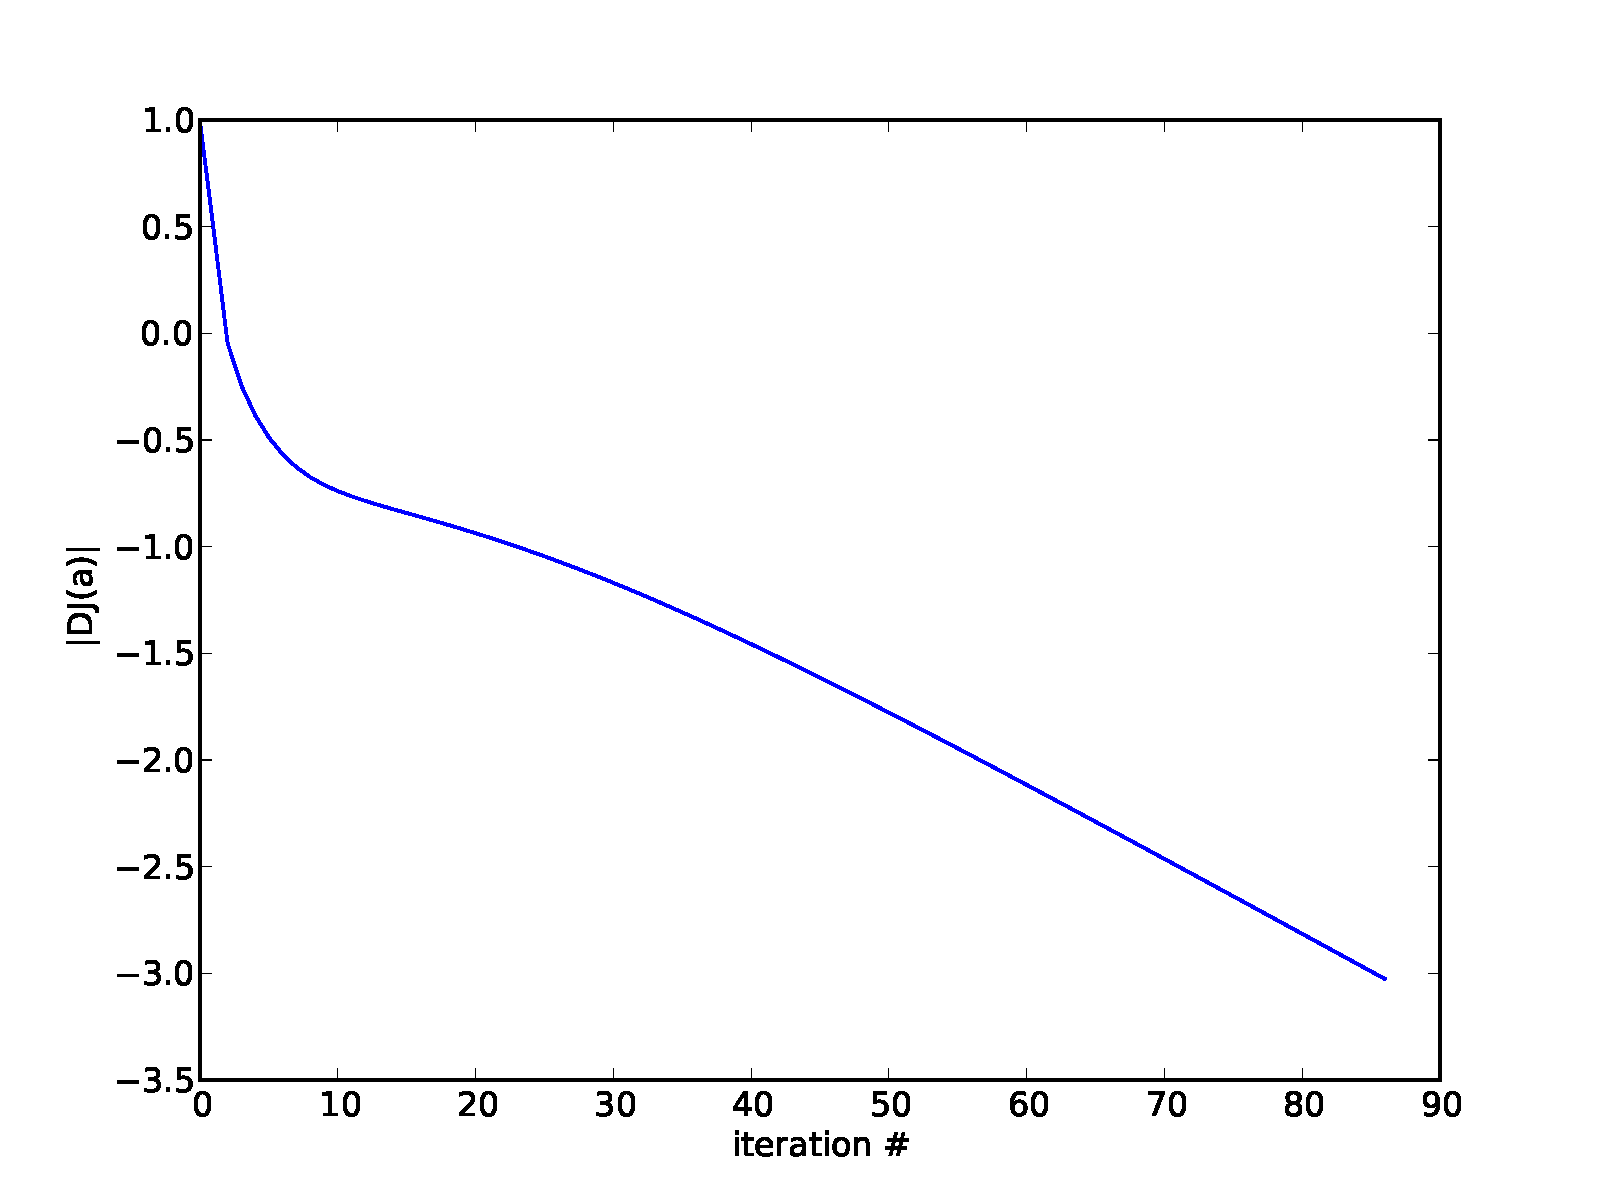
\includegraphics[width = 250pt]{convergence.pdf}
\caption{Convergence of optimization algorithm. The convergence rate appears to be linear.  \textbf{(NOTE I''LL MAKE THIS FIGURE NICER'')}}
\label{fig-conv}
\end{figure}
Earlier, we simulated the loop's dynamics for spring constant values of $\kappa_\theta = \kappa_\psi = 20$.  Now, we wish to identify these spring constants using only position measurements that were taken at the frame where the force was applied, frame $L_{3,e}$.  It is reasonable to assume a robotic manipulator could measure its end effector's position as it manipulates an object.  

In order to optimally identify the parameters, the cost function, $J_d$ must reflect the measurement data.  Let $w_{k,meas}$ be the measured position of the end effector at time $t_k$, which corresponds to the origin of $L_{3,e}$ for the measured loop.  The optimization problem is to find the parameters $a = [\kappa_\theta,\kappa_\psi]^T$ which correspond to a simulation for which the origin of $L_{3,e}$ best matches $w_{k,meas}$. Therefore, we set the running and terminal costs to: $\ell_d(q_k,a) = 1/2(w_k-w_{k,meas})^T(w_k-w_{k,meas})$ and $m_d(q_{k_f},a) =  1/2(w_{k_f}-w_{k_F,meas})^T(w_{k}-w_{{k_f},meas})$ where $w_k$ is the origin of the frame $L_{3,e}$ for configuration $q_k$.

Starting with an initial guess of $a = [10, 25]^T$, we execute steepest descent with an Armijo line search which has parameters $\alpha = \beta = 0.4$ \cite{armijo}.  After $86$ iterations, the algorithm terminates with gradient norm $|DJ_d(a)| < 10^{-3}$.  The parameters are identified as $[19.9997,  20.0120]^T$.  The convergence is shown in Fig.~\ref{fig-conv}.




\bibliographystyle{plain}
\bibliography{param_opts_cites}

\end{document}